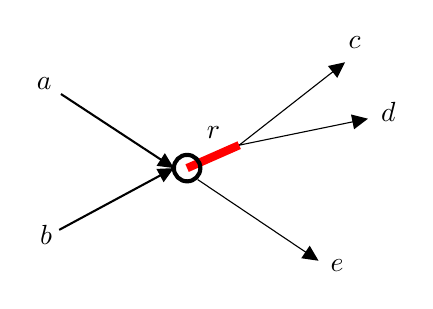
\begin{tikzpicture}[x=0.75pt,y=0.75pt,yscale=-0.85,xscale=0.85]
%uncomment if require: \path (0,146); %set diagram left start at 0, and has height of 146

%Straight Lines [id:da16249976297719293] 
\draw [line width=0.75]    (23.5,37) -- (85.83,77.9) ;
\draw [shift={(87.5,79)}, rotate = 213.27] [fill={rgb, 255:red, 0; green, 0; blue, 0 }  ][line width=0.75]  [draw opacity=0] (8.93,-4.29) -- (0,0) -- (8.93,4.29) -- cycle    ;

%Straight Lines [id:da772784293523332] 
\draw [line width=0.75]    (22.5,114) -- (85.74,79.95) ;
\draw [shift={(87.5,79)}, rotate = 511.7] [fill={rgb, 255:red, 0; green, 0; blue, 0 }  ][line width=0.75]  [draw opacity=0] (8.93,-4.29) -- (0,0) -- (8.93,4.29) -- cycle    ;

%Straight Lines [id:da9613918488192326] 
\draw [color={rgb, 255:red, 255; green, 0; blue, 0 }  ,draw opacity=1 ][line width=3]    (95,79) -- (124.5,66) ;


%Shape: Circle [id:dp6094178436022282] 
\draw  [line width=1.5]  (87.5,79) .. controls (87.5,74.86) and (90.86,71.5) .. (95,71.5) .. controls (99.14,71.5) and (102.5,74.86) .. (102.5,79) .. controls (102.5,83.14) and (99.14,86.5) .. (95,86.5) .. controls (90.86,86.5) and (87.5,83.14) .. (87.5,79) -- cycle ;
%Straight Lines [id:da9688539202688002] 
\draw    (124.5,66) -- (182.93,20.23) ;
\draw [shift={(184.5,19)}, rotate = 501.93] [fill={rgb, 255:red, 0; green, 0; blue, 0 }  ][line width=0.75]  [draw opacity=0] (8.93,-4.29) -- (0,0) -- (8.93,4.29) -- cycle    ;

%Straight Lines [id:da9340506100154327] 
\draw    (124.5,66) -- (195.54,51.4) ;
\draw [shift={(197.5,51)}, rotate = 528.39] [fill={rgb, 255:red, 0; green, 0; blue, 0 }  ][line width=0.75]  [draw opacity=0] (8.93,-4.29) -- (0,0) -- (8.93,4.29) -- cycle    ;

%Straight Lines [id:da7562683529308978] 
\draw    (101,85.5) -- (167.84,130.39) ;
\draw [shift={(169.5,131.5)}, rotate = 213.88] [fill={rgb, 255:red, 0; green, 0; blue, 0 }  ][line width=0.75]  [draw opacity=0] (8.93,-4.29) -- (0,0) -- (8.93,4.29) -- cycle    ;


% Text Node
\draw (14,31) node  [align=left] {$a$};
% Text Node
\draw (15,117) node  [align=left] {$b$};
% Text Node
\draw (190,8) node  [align=left] {$c$};
% Text Node
\draw (209,47) node  [align=left] {$d$};
% Text Node
\draw (180,134) node  [align=left] {$e$};
% Text Node
\draw (110,59) node  [align=left] {$r$};


\end{tikzpicture}